\documentclass{standalone}
\usepackage{tikz}
\usepackage{ctex,siunitx}
\setCJKmainfont{Noto Serif CJK SC}
\usepackage{tkz-euclide}
\usepackage{amsmath,upgreek}
\usetikzlibrary{patterns, calc,3d}
\usetikzlibrary {decorations.pathmorphing,decorations.pathreplacing,decorations.shapes}
\begin{document}
\small
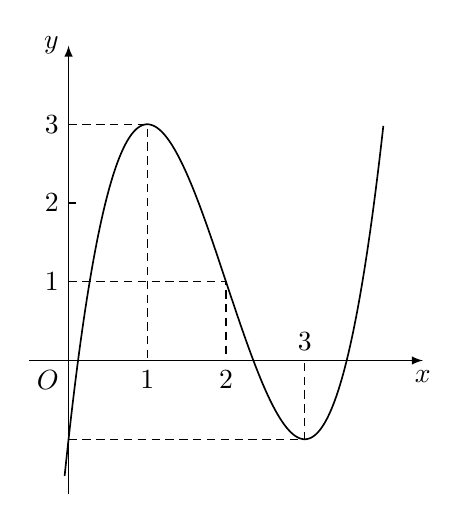
\begin{tikzpicture}[>=latex,scale=1.0]
  \draw[->](-0.5,0)--(4.5,0)node[below]{$x$};
  \draw[->](0,-1.7)--(0,4)node[left]{$y$};
  \node at (0,0)[below left]{$O$};
  \draw[samples=200,domain=-0.05:4,semithick]plot(\x,{\x*\x*\x-6*\x*\x+9*\x-1});
  \draw[densely dashed](0,-1)--(3,-1)--(3,0)node[above]{3};
  \draw[densely dashed](0,3)node[left]{3}--(1,3)--(1,0)node[below]{1};
  \draw[densely dashed](0,1)node[left]{1}--(2,1)--(2,0)node[below]{2};
  \draw(0.1,2)--(0,2)node[left]{2};
\end{tikzpicture}
\end{document}